%%%
%%% Preamble
%%%
\documentclass[12pt,english]{kuthesis}
\usepackage{mathptmx}
\renewcommand{\sfdefault}{lmss}
\renewcommand{\ttdefault}{lmtt}
\usepackage[T1]{fontenc}
\usepackage[utf8]{inputenc}
\usepackage{geometry}
\geometry{verbose,tmargin=1in,bmargin=1in,lmargin=1in,rmargin=1in}
\setcounter{secnumdepth}{3}
\setcounter{tocdepth}{3}
\usepackage{color}
\usepackage{babel}
\usepackage{url}
\usepackage{graphicx}
\usepackage{setspace}
\usepackage{esint}
\usepackage[authoryear]{natbib}
\doublespacing
\usepackage[unicode=true,
 bookmarks=true,bookmarksnumbered=false,bookmarksopen=false,
 breaklinks=true,pdfborder={0 0 0},pdfborderstyle={},backref=false,colorlinks=true]
 {hyperref}
\hypersetup{pdftitle={University of Kansas Thesis Template},
 pdfauthor={Anonymous},
 pdfsubject={A Thesis},
 urlcolor={black},citecolor={black},allcolors={black}}

%% These additions are made to make the template play nice with pandoc
\providecommand{\tightlist}{%
  \setlength{\itemsep}{0pt}\setlength{\parskip}{0pt}}
\usepackage{fancyvrb}
\let\iint=\relax
\let\iiint=\relax
\let\iiiint=\relax
\let\idotsint=\relax
\usepackage{amsmath}
\DefineVerbatimEnvironment{Highlighting}{Verbatim}{commandchars=\\\{\}\linespread{1}\normalfont\ttfamily}
\usepackage{framed}
\definecolor{shadecolor}{RGB}{248,248,248}
\newenvironment{Shaded}{\begin{snugshade}}{\end{snugshade}}
\newcommand{\KeywordTok}[1]{\textcolor[rgb]{0.13,0.29,0.53}{\textbf{#1}}}
\newcommand{\DataTypeTok}[1]{\textcolor[rgb]{0.13,0.29,0.53}{#1}}
\newcommand{\DecValTok}[1]{\textcolor[rgb]{0.00,0.00,0.81}{#1}}
\newcommand{\BaseNTok}[1]{\textcolor[rgb]{0.00,0.00,0.81}{#1}}
\newcommand{\FloatTok}[1]{\textcolor[rgb]{0.00,0.00,0.81}{#1}}
\newcommand{\ConstantTok}[1]{\textcolor[rgb]{0.00,0.00,0.00}{#1}}
\newcommand{\CharTok}[1]{\textcolor[rgb]{0.31,0.60,0.02}{#1}}
\newcommand{\SpecialCharTok}[1]{\textcolor[rgb]{0.00,0.00,0.00}{#1}}
\newcommand{\StringTok}[1]{\textcolor[rgb]{0.31,0.60,0.02}{#1}}
\newcommand{\VerbatimStringTok}[1]{\textcolor[rgb]{0.31,0.60,0.02}{#1}}
\newcommand{\SpecialStringTok}[1]{\textcolor[rgb]{0.31,0.60,0.02}{#1}}
\newcommand{\ImportTok}[1]{#1}
\newcommand{\CommentTok}[1]{\textcolor[rgb]{0.56,0.35,0.01}{\textit{#1}}}
\newcommand{\DocumentationTok}[1]{\textcolor[rgb]{0.56,0.35,0.01}{\textbf{\textit{#1}}}}
\newcommand{\AnnotationTok}[1]{\textcolor[rgb]{0.56,0.35,0.01}{\textbf{\textit{#1}}}}
\newcommand{\CommentVarTok}[1]{\textcolor[rgb]{0.56,0.35,0.01}{\textbf{\textit{#1}}}}
\newcommand{\OtherTok}[1]{\textcolor[rgb]{0.56,0.35,0.01}{#1}}
\newcommand{\FunctionTok}[1]{\textcolor[rgb]{0.00,0.00,0.00}{#1}}
\newcommand{\VariableTok}[1]{\textcolor[rgb]{0.00,0.00,0.00}{#1}}
\newcommand{\ControlFlowTok}[1]{\textcolor[rgb]{0.13,0.29,0.53}{\textbf{#1}}}
\newcommand{\OperatorTok}[1]{\textcolor[rgb]{0.81,0.36,0.00}{\textbf{#1}}}
\newcommand{\BuiltInTok}[1]{#1}
\newcommand{\ExtensionTok}[1]{#1}
\newcommand{\PreprocessorTok}[1]{\textcolor[rgb]{0.56,0.35,0.01}{\textit{#1}}}
\newcommand{\AttributeTok}[1]{\textcolor[rgb]{0.77,0.63,0.00}{#1}}
\newcommand{\RegionMarkerTok}[1]{#1}
\newcommand{\InformationTok}[1]{\textcolor[rgb]{0.56,0.35,0.01}{\textbf{\textit{#1}}}}
\newcommand{\WarningTok}[1]{\textcolor[rgb]{0.56,0.35,0.01}{\textbf{\textit{#1}}}}
\newcommand{\AlertTok}[1]{\textcolor[rgb]{0.94,0.16,0.16}{#1}}
\newcommand{\ErrorTok}[1]{\textcolor[rgb]{0.64,0.00,0.00}{\textbf{#1}}}
\newcommand{\NormalTok}[1]{#1}
\usepackage{float}
%% end of additions

\makeatletter
\usepackage{dcolumn}
\usepackage{booktabs}

\title{Writing Theses and Dissertations with jayhawkdown}
\author{W. Jake Thompson}
\priorcreds{B.S. Behavioral Neuroscience, University of Kansas, 2014 \\ Ph.D.~Educational Psychology, University of Kansas, 2018}

\dept{Educational Psychology}
\degreetitle{Doctor of Philosophy}
\papertype{Dissertation}
\committee{Committee Member \#1}{Committee Member \#2}{Committee Member \#3}{Committee Member \#4}{Committee Member \#5}{}{}
\role{Chairperson}{}{}{}{Outside member}{}{}

\@printd@testrue
\datedefended{February 16, 2020}
\dateapproved{February 16, 2020}

\@ifundefined{showcaptionsetup}{}{%
  \PassOptionsToPackage{caption=false}{subfig}}
\usepackage{subfig}
\makeatother

\usepackage{listings}
\renewcommand{\lstlistingname}{\inputencoding{latin9}Listing}

\begin{document}
\begin{romanpages}

\maketitle
  \begin{abstract}
    The \textbf{jayhawkdown} package can be used to write theses and dissertations in R Markdown that meet the formatting requirements of the University of Kansas. By harnessing the power R Markdown, we are able to write prose in the simplified markdown language and render the output as a PDF document. Thus, we get the benefits of \LaTeX~without having to actually write any \LaTeX~code. R Markdown also allows analysis code to be included directly in the document. This means the results, figures, and tables can be dynamically populated directly in the paper, making everything completely reproducible. Finally, because \textbf{jayhawkdown} is built on top of the \textbf{bookdown} package, it's also possible to render your document to other output formats, such as a website.
    
    \emph{Keywords}. R Markdown, Thesis, Dissertation, LaTeX, Kansas
  \end{abstract}

  \begin{acknowledgementslong}
    The \textbf{jayhawkdown} package would not be possible without the work of many others. First, Yihui Xie, for creating the \href{https://yihui.org/knitr/}{\textbf{knitr}} package, the \href{https://github.com/rstudio/rmarkdown}{\textbf{rmarkdown}} package with J. J. Allaire, and the \href{https://github.com/rstudio/bookdown}{\textbf{bookdown}} package. Without these three packages, \textbf{jayhawkdown} could not exist. Second, Chester Ismay for creating the \href{https://github.com/ismayc/thesisdown}{\textbf{thesisdown}} package for Reed College, which served as the direct inspiration and template for this package. Third, Paul Johnson for creating the original University of Kansas \LaTeX~template, which has been adpated here. Finally, to my own dissertation committee: Neal Kingston, Jonathan Templin, Billy Skorupski, Brooke Nash, and Paul Johnson, for being patient as I procrastinated my own dissertation to write this package, just so I could avoid \LaTeX.
  \end{acknowledgementslong}
\tableofcontents{}

\listoffigures

\listoftables

\end{romanpages}

\hypertarget{using-jayhawkdown}{%
\chapter{Using jayhawkdown}\label{using-jayhawkdown}}

The \textbf{jayhawkdown} package is designed to provide a template for writing theses and dissertations at the University of Kansas using \textbf{rmarkdown} (Allaire et al., \protect\hyperlink{ref-R-rmarkdown}{2020}) and \textbf{bookdown} (Xie, \protect\hyperlink{ref-R-bookdown}{2020}\protect\hyperlink{ref-R-bookdown}{a}). This chapter walks you through how to edit and alter the template to fit your needs.

\hypertarget{getting-started}{%
\section{Getting started}\label{getting-started}}

The structure of your thesis or dissertation is defined the \texttt{\_bookdown.yml} file. The most important part of this file is the \texttt{rmd\_files:} listing at the top. This defines which documents to include and the order in which to include them. The first file must be template R Markdown file that was generated in the main directory when the template was opened. For example, if you named the directory ``skeleton'' when the template was opened, you should see a \texttt{skeleton.rmd} document in the main directory. After that file, all documents can be moved and/or deleted to your liking. The exception is the references file. I can be moved into any order you chose (e.g., after the appendix instead of before), but \textbf{DO NOT} delete this file. It contains several formatting options and tags to ensure that the references follow APA style and actually appear where you are intending them to.

In the main R Markdown file, you will see some YAML metadata at the top that is needed to create the dissertation. Edit the fields in the \texttt{\#\#\#\ Required\ Information} section so that they reflect your document. If fields are not needed (e.g., you have less than 7 people on your committee), simply delete those lines. The next section is \texttt{\#\#\#\ Rendering\ Options}. Although these can be edited, this should only be done if you know what you are doing and have a very good reason for doing so. The final section is \texttt{\#\#\#\ Pretext\ Sections}. This points to the abstract and acknowledgements files, which are located in the \texttt{pre/} folder.

\hypertarget{adding-chapters}{%
\section{Adding chapters}\label{adding-chapters}}

To add a new chapter, simply create a new R Markdown document and add it the \texttt{chapters/} folder and the \texttt{\_bookdown.yml} file. It's that easy!

\hypertarget{creating-your-documents}{%
\section{Creating your documents}\label{creating-your-documents}}

To create a PDF version of your thesis or dissertation, press the knit button at the top of the RStudio editor. If you aren't using RStudio, you can use \texttt{bookdown::render\_book("index.Rmd",\ "jayhawkdown::thesis\_pdf")}, where \texttt{skeleton.rmd} is the name of the R Markdown document that include the YAML metadata. This will create your document at \texttt{\_book/thesis.pdf}. To change the name of this file, you can edit the \texttt{book\_filename} in \texttt{\_bookdown.yml}.

\hypertarget{writing-in-r-markdown}{%
\chapter{Writing in R Markdown}\label{writing-in-r-markdown}}

R Markdown documents use the markdown language to format plain text in the final document. The \textbf{bookdown} package (Xie, \protect\hyperlink{ref-R-bookdown}{2020}\protect\hyperlink{ref-R-bookdown}{a}) extends the R Markdown language to include additional features. For a full description of all the features available to you, see the \href{https://bookdown.org/yihui/bookdown/components.html}{Components} chapter of the \textbf{bookdown} book (Xie, \protect\hyperlink{ref-bookdown}{2016}). In this chapter I'll highlight some of the key features that are most likely to be used.

\hypertarget{format}{%
\section{Formatting text}\label{format}}

Font can be made \textbf{bold} or \emph{italic} by using asterisks or underscores. Make words bold by using two (i.e., \texttt{**bold**} or \texttt{\_\_bold\_\_}) and italic using one (i.e., \texttt{*italic*} or \texttt{\_italic\_}).

You can create headings by using the \# sign. Each \# is an additional level.

\begin{Shaded}
\begin{Highlighting}[]
\FunctionTok{# Chapter Name}

\FunctionTok{## Section Name}

\FunctionTok{### Subsection}
\end{Highlighting}
\end{Shaded}

You can also create bulleted or numbered lists. Bulleted lists can be created with \texttt{*}, \texttt{-}, or \texttt{+}. For example,

\begin{Shaded}
\begin{Highlighting}[]
\NormalTok{- }\FloatTok{item one}
\FloatTok{- item two}
\FloatTok{    - sub item}
\FloatTok{- item three}
\end{Highlighting}
\end{Shaded}

Yields the following list:

\begin{itemize}
\tightlist
\item
  item one
\item
  item two

  \begin{itemize}
  \tightlist
  \item
    sub item
  \end{itemize}
\item
  item three
\end{itemize}

Similarly,

\begin{Shaded}
\begin{Highlighting}[]
\NormalTok{1. }\FloatTok{item one}
\FloatTok{2. item two}
\FloatTok{    1. sub item}
\FloatTok{3. item three}
\end{Highlighting}
\end{Shaded}

Yields a numbered list:

\begin{enumerate}
\def\labelenumi{\arabic{enumi}.}
\tightlist
\item
  item one
\item
  item two

  \begin{enumerate}
  \def\labelenumii{\arabic{enumii}.}
  \tightlist
  \item
    sub item
  \end{enumerate}
\item
  item three
\end{enumerate}

You can also add code text that will be rendered in a typewriter font. This can be done inline by using single back ticks. You can also put an entire block of text in code by use three back ticks before and after the block begins and ends.

\hypertarget{latex-equations}{%
\section{Latex Equations}\label{latex-equations}}

Equations can be added seemlessly by using \LaTeX~syntax. For example:

\begin{Shaded}
\begin{Highlighting}[]
\NormalTok{$$}
\NormalTok{P(X_\{ij\} = 1|\textbackslash{}theta) = \textbackslash{}frac\{1\}\{1-e^\{(-a_j (\textbackslash{}theta_i-b_j))\}\}}
\NormalTok{$$}
\end{Highlighting}
\end{Shaded}

Yields the following equaiton:
\[
P(X_{ij} = 1|\theta) = \frac{1}{1-e^{(-a_j (\theta_i-b_j))}}
\]

Double dollar signs will center the equation on its own line. A single dollar sign before and after will include the equation inline (i.e., \(A = \pi r^2\)).

\hypertarget{cross-references}{%
\section{Cross References}\label{cross-references}}

One of the extensions provided by the \textbf{bookdown} package is easy cross references. To reference a figure, simply add the \texttt{fig.cap} arugment as a chunk option with a relevant caption.

\begin{Shaded}
\begin{Highlighting}[]
\KeywordTok{library}\NormalTok{(ggplot2)}
\NormalTok{mtcars <-}\StringTok{ }\KeywordTok{read.csv}\NormalTok{(}\StringTok{"data/mtcars.csv"}\NormalTok{, }\DataTypeTok{stringsAsFactors =} \OtherTok{FALSE}\NormalTok{, }\DataTypeTok{row.names =} \DecValTok{1}\NormalTok{)}

\KeywordTok{ggplot}\NormalTok{(mtcars, }\KeywordTok{aes}\NormalTok{(disp, mpg, }\DataTypeTok{colour =} \KeywordTok{factor}\NormalTok{(cyl))) }\OperatorTok{+}\StringTok{ }
\StringTok{  }\KeywordTok{geom_point}\NormalTok{()}
\end{Highlighting}
\end{Shaded}

\begin{figure}

{\centering 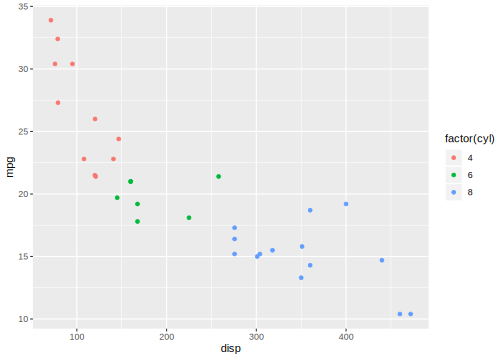
\includegraphics[width=0.8\linewidth]{jayhawkdown_files/figure-latex/plot-1} 

}

\caption{Here is a figure caption to describe this graph}\label{fig:plot}
\end{figure}

This will automatically number the figure and add the caption. Figure \ref{fig:plot} can then be referenced using \texttt{\textbackslash{}@ref(fig:plot)}, where \texttt{plot} is the name of the code chunk. All figures that are generated in R will be saved to the \texttt{figure} directory. Alternatively, you can add your own images to \texttt{figure/} and add them using \texttt{knitr::include\_graphics()}.

You can similarly add references to tables. Table \ref{tab:tab-summary} is created using \texttt{knitr::kable()}, which allows a caption to be specified. This will number the table, which then can be referenced using similar syntax (i.e., \texttt{\textbackslash{}@ref(tab:tab-summary))}. There are many different packages that will create tables for you, each with their own strengths and weaknesses. For example the \textbf{rockchalk} (Johnson, \protect\hyperlink{ref-R-rockchalk}{2016}) and \textbf{texreg} (Leifeld, \protect\hyperlink{ref-R-texreg}{2017}) packages will both create APA style regression tables, which can be modified to include cross references.

\begin{Shaded}
\begin{Highlighting}[]
\KeywordTok{library}\NormalTok{(dplyr)}

\NormalTok{mtcars }\OperatorTok
\StringTok{  }\KeywordTok{group_by}\NormalTok{(cyl) }\OperatorTok
\StringTok{  }\KeywordTok{select}\NormalTok{(cyl}\OperatorTok{:}\NormalTok{hp) }\OperatorTok
\StringTok{  }\KeywordTok{summarize_all}\NormalTok{(mean) }\OperatorTok
\StringTok{  }\NormalTok{knitr}\OperatorTok{::}\KeywordTok{kable}\NormalTok{(}\DataTypeTok{caption =} \StringTok{"Here's a table of summary statistics"}\NormalTok{,}
    \DataTypeTok{booktabs =} \OtherTok{TRUE}\NormalTok{)}
\end{Highlighting}
\end{Shaded}

\begin{table}

\caption{\label{tab:tab-summary}Here's a table of summary statistics}
\centering
\begin{tabular}[t]{rrr}
\toprule
cyl & disp & hp\\
\midrule
4 & 105.1364 & 82.63636\\
6 & 183.3143 & 122.28571\\
8 & 353.1000 & 209.21429\\
\bottomrule
\end{tabular}
\end{table}

The third type of cross referencing is for equations. This requires a little bit more work. Recall that to create an equation above we used the following syntax:

\begin{Shaded}
\begin{Highlighting}[]
\NormalTok{$$}
\NormalTok{P(X_\{ij\} = 1|\textbackslash{}theta) = \textbackslash{}frac\{1\}\{1-e^\{(-a_j (\textbackslash{}theta_i-b_j))\}\}}
\NormalTok{$$}
\end{Highlighting}
\end{Shaded}

In order to create a cross reference, we have to define the \LaTeX~equation and then add the reference:

\begin{Shaded}
\begin{Highlighting}[]
\NormalTok{\textbackslash{}begin\{equation\}}
\NormalTok{  P(X_\{ij\} = 1|\textbackslash{}theta) = \textbackslash{}frac\{1\}\{1-e^\{(-a_j (\textbackslash{}theta_i-b_j))\}\}}
\NormalTok{  (\textbackslash{}#eq:irt-model)}
\NormalTok{\textbackslash{}end\{equation\}}
\end{Highlighting}
\end{Shaded}

\begin{equation}
  P(X_{ij} = 1|\theta) = \frac{1}{1-e^{(-a_j (\theta_i-b_j))}}
  \label{eq:irt-model}
\end{equation}

That code will render the equation and give it a number, which can then be referenced using the label provided (i.e., \texttt{\textbackslash{}@ref(eq:irt-model)} will create the reference for equation \eqref{eq:irt-model}).

The final type of cross referencing that I'll discuss here is referencing sections of the paper. This is done by using the section headings (i.e., we talked about \LaTeX~equations in section \ref{latex-equations}). By default, references for section headings are defined by the section name. For example to reference the section on equations using \LaTeX, I use \texttt{\textbackslash{}@ref(latex-equations)}, because the name of the section is ``Latex Equations''. However, you can also define your own labels by add \texttt{\{\#label\}} after the section heading. For example, the section heading for section \ref{format} looks like this:

\begin{Shaded}
\begin{Highlighting}[]
\FunctionTok{## Formatting text \{#format\}}
\end{Highlighting}
\end{Shaded}

So to create a reference for this section I can use \texttt{\textbackslash{}@ref(format)}. You can also create links. For example, the following code will create a link where the word ``instructions'' links to the ``Getting started'' section in Chapter \ref{using-jayhawkdown}:

\begin{Shaded}
\begin{Highlighting}[]
\OtherTok{[instructions][Getting started]}
\end{Highlighting}
\end{Shaded}

This template comes with \protect\hyperlink{getting-started}{instructions}. However, it is probably more useful to reference the specific section number using the \texttt{\textbackslash{}@ref(getting-started)} syntax.

\hypertarget{citations}{%
\section{Citations}\label{citations}}

Citations are also straightforward to add in the markdown language. All that is required is a BibTeX file to be placed in the \texttt{bib/} directory. You can add as many BibTeX files as you would like, as long as you list them in the \texttt{bibliography:} options under the YAML metadata in the main R Markdown document. To reference a citation in the text use \texttt{{[}@reference-key{]}} or \texttt{@reference-key}, where \texttt{reference-key} is the name given to the reference in the BibTeX file. Putting the key inside of brackets will make the entire citation appear within parentheses, whereas no brackets will put only the year in parentheses.

\begin{itemize}
\tightlist
\item
  \texttt{{[}@bookdown{]}} renders as (Xie, \protect\hyperlink{ref-bookdown}{2016})
\item
  \texttt{@bookdown} renders as Xie (\protect\hyperlink{ref-bookdown}{2016})
\end{itemize}

You can include multiple citations within a single set of brackets by separating them with a semicolon. Finally, you can suppress the author's name by using a \texttt{-} sign before the key (i.e., \texttt{{[}-@bookdown{]}}).

By default, references for all R packages that are loaded with your session are will be written to \texttt{bib/packages.bib}. They key for packages will be ``R-packagename''. For example, I used \textbf{ggplot} to generate Figure \ref{fig:plot}, so I could cite the package by using \texttt{{[}@R-ggplot2{]}} (Wickham et al., \protect\hyperlink{ref-R-ggplot2}{2019}).

All citations in the body of your document will automatically be included in the references chapter. If you would like to include additional references without citing them in your text, add the keys to the \texttt{nocite:} field of the YAML metadata.

\hypertarget{references}{%
\chapter*{References}\label{references}}
\addcontentsline{toc}{chapter}{References}

\setlength{\parindent}{-15pt}
\setlength{\leftskip}{15pt}

\noindent

\hypertarget{refs}{}
\leavevmode\hypertarget{ref-R-rmarkdown}{}%
Allaire, J., Xie, Y., McPherson, J., Luraschi, J., Ushey, K., Atkins, A., Wickham, H., Cheng, J., Chang, W., \& Iannone, R. (2020). \emph{Rmarkdown: Dynamic documents for r}. \url{https://CRAN.R-project.org/package=rmarkdown}

\leavevmode\hypertarget{ref-R-rockchalk}{}%
Johnson, P. E. (2016). \emph{Rockchalk: Regression estimation and presentation}. \url{https://CRAN.R-project.org/package=rockchalk}

\leavevmode\hypertarget{ref-R-texreg}{}%
Leifeld, P. (2017). \emph{Texreg: Conversion of r regression output to latex or html tables}. \url{https://CRAN.R-project.org/package=texreg}

\leavevmode\hypertarget{ref-R-jayhawkdown}{}%
Thompson, W. J. (2020). \emph{Jayhawkdown: A bookdown template for university of kansas dissertations}.

\leavevmode\hypertarget{ref-R-ggplot2}{}%
Wickham, H., Chang, W., Henry, L., Pedersen, T. L., Takahashi, K., Wilke, C., Woo, K., \& Yutani, H. (2019). \emph{Ggplot2: Create elegant data visualisations using the grammar of graphics}. \url{https://CRAN.R-project.org/package=ggplot2}

\leavevmode\hypertarget{ref-bookdown}{}%
Xie, Y. (2016). \emph{bookdown: Authoring Books and Technical Documents with R Markdown} (1st ed.). Chapman \& Hall.

\leavevmode\hypertarget{ref-R-bookdown}{}%
Xie, Y. (2020a). \emph{Bookdown: Authoring books and technical documents with r markdown}. \url{https://CRAN.R-project.org/package=bookdown}

\leavevmode\hypertarget{ref-R-knitr}{}%
Xie, Y. (2020b). \emph{Knitr: A general-purpose package for dynamic report generation in r}. \url{https://CRAN.R-project.org/package=knitr}

\setlength{\parindent}{15pt}
\setlength{\leftskip}{0pt}

\hypertarget{appendix-appendix}{%
\appendix}


\hypertarget{something-important}{%
\chapter{Something important}\label{something-important}}

You can put an appendix (or multiple appendices) here. Each appendix can be added as a separate R Markdown document, just like a chapter, and placed in the desired order in the \texttt{\_bookdown.yml} file. The only constraint is that the first appendix must begin with a special tag.

\begin{Shaded}
\begin{Highlighting}[]
\FunctionTok{# (APPENDIX) Appendix \{-\}}

\FunctionTok{# Name of Appendix A}
\end{Highlighting}
\end{Shaded}

The first line sets a flag to indicate that the appendices are starting. This will make the following chapters be labeled Appendix A, Appendix B, etc., rather than continuing the chapter numbering from the main body of the thesis.

\end{document}
